\chapter{Experiment}
In this experiment an optical transmission system was used. At first the Power-Voltage characteristic of a Mach-Zehnder modulator was recorded to find the quadrature point and determine the operation point. In the second setup the extinction ratio of the modulator was analyzed and optimized and after that the Q-factor was measured. In the last setup a PRBS was transmitted and received and the BER was measured. With this the receiver sensitivity should be estimated.  

\section{Setup A: Estimation of the quadrature point of the MZI modulator}


\begin{figure}[t]%
\centering
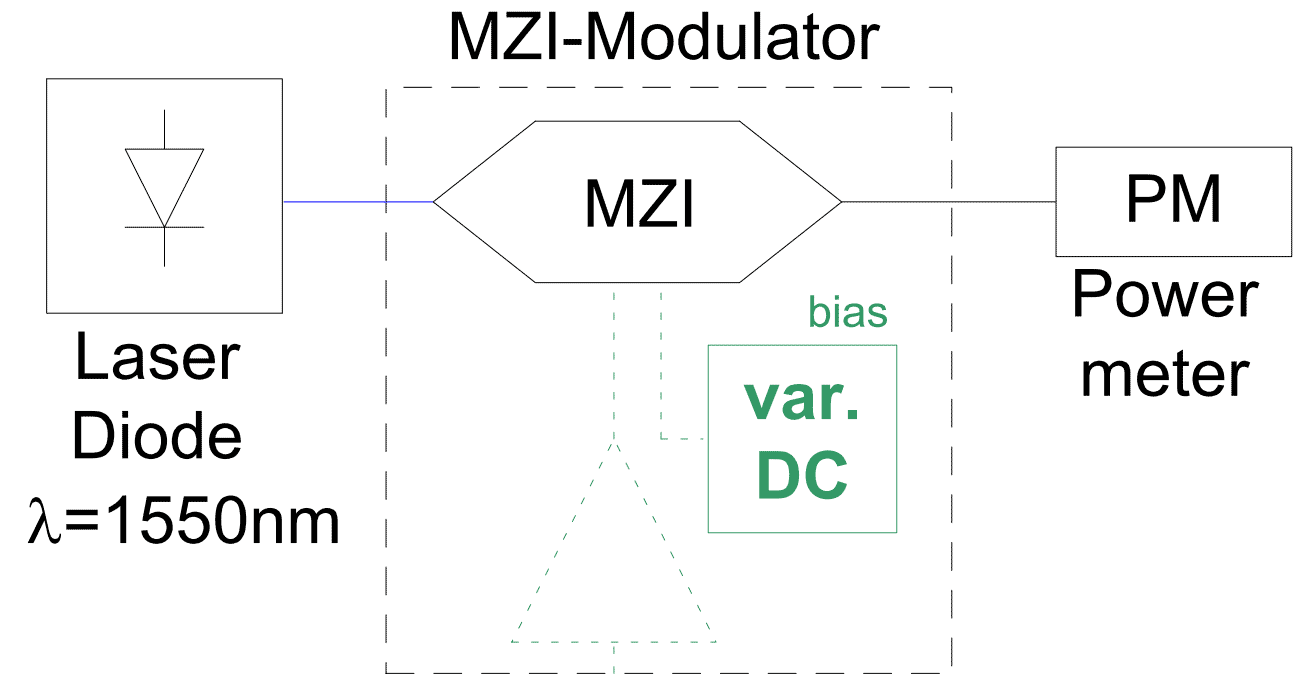
\includegraphics[width=.5\columnwidth]{Grafiken/SetupA.png}%
\caption{Setup A}%
\label{fig:A_setup}%
\end{figure}



To calculate the quadrature point of the used MZI modulator the setup shown in figure \ref{fig:A_setup}\footnote[3]{Luca Alloatti, Materials for the preparation of OKT lab 8} was used. A laser source with an output wavelength of 1550~nm and an output power of 0~dBm were connected to an MZI modulator. The output of the MZI modulator was connected to a power meter. The modulator was biased over a variable DC voltage.

The DC voltage was swept from -4.8~V to 5.1~V in steps of 0.3~V. At every point the output power of the MZM was measured.

\begin{figure}%
\centering
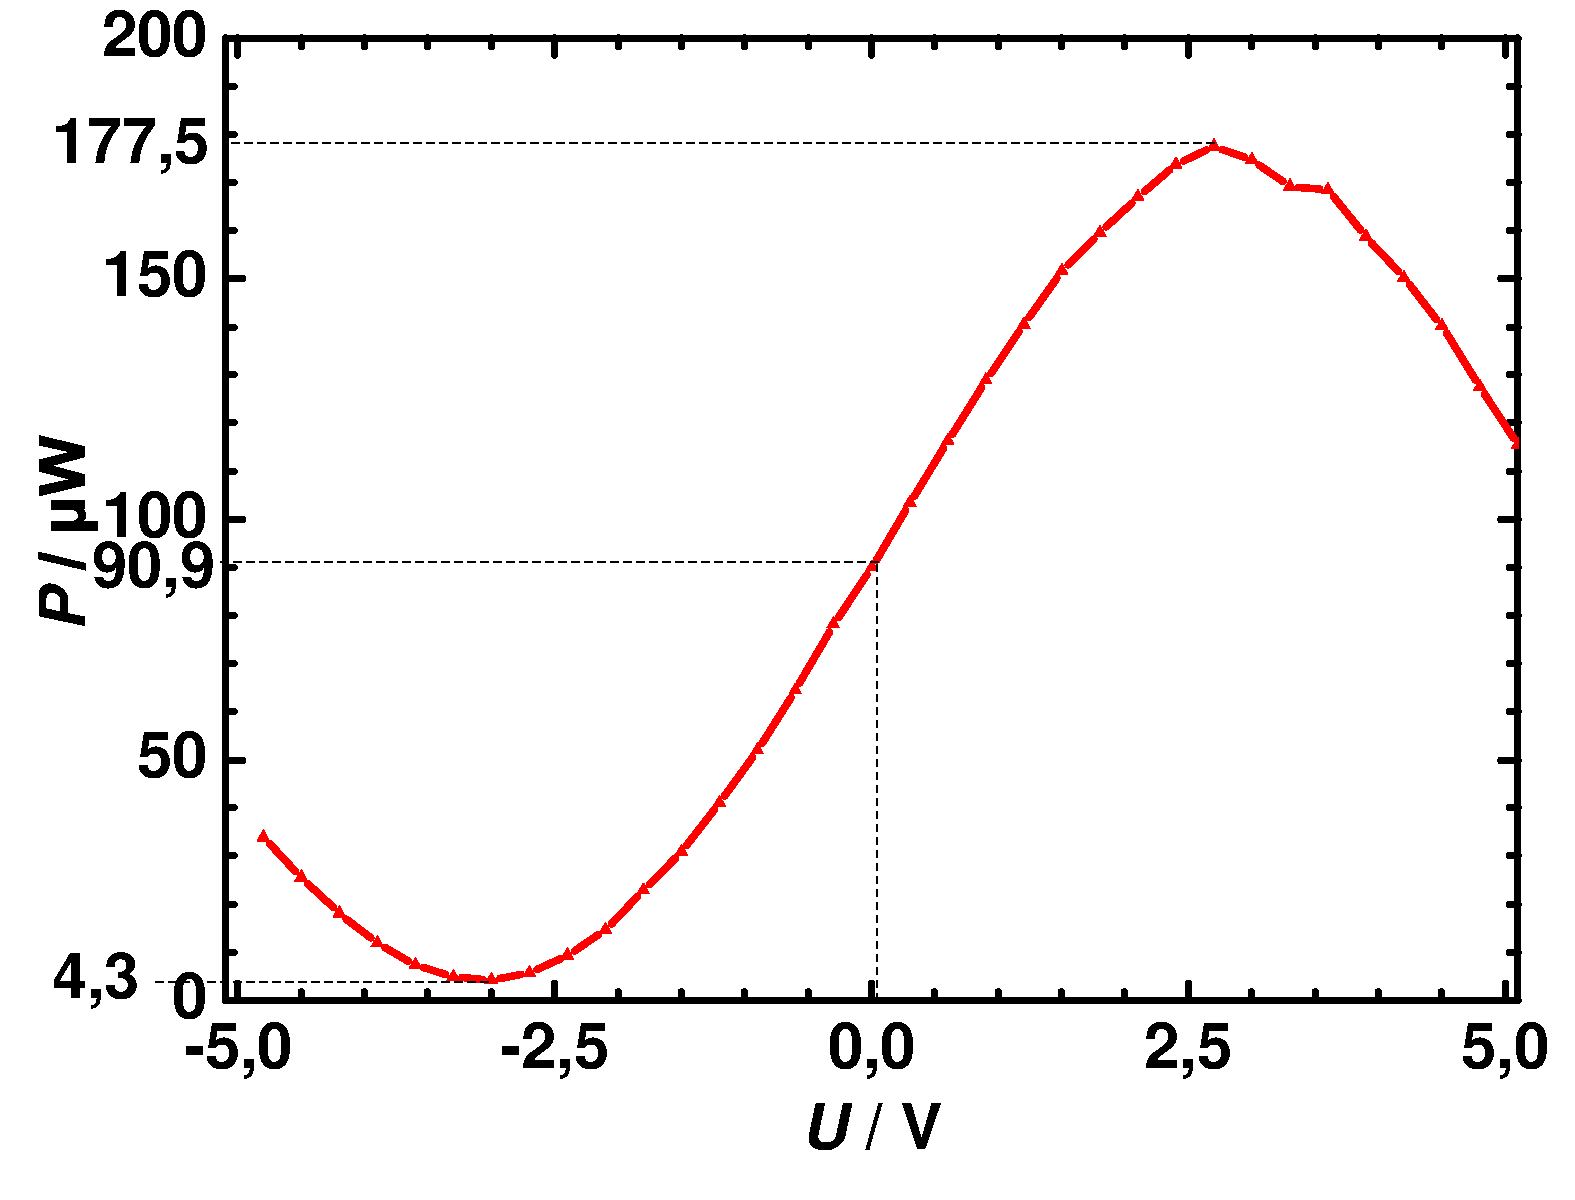
\includegraphics[width=.6\columnwidth]{Grafiken/A_quadratur.pdf}%
\caption{$P$/$U$ characteristic of the MZM.}%
\label{fig:A_quadratur}%
\end{figure}

Figure \ref{fig:A_quadratur} shows the recorded $P$/$U$ curve. It shows a good accordance to the squared sine $P$/$U$ curve of a theoretical MZI modulator.
The maximum optical output power of the MZI is at 2.5~V with 177.5~$\upmu$W. The minimal optical output power is at -3.0~V with 4.3~$\upmu$W. With this the quadrature point can be calculated to be at

\begin{equation}
P\i{out,quadrature}=\frac{177.5~\upmu \mathrm{W}+4.3~\upmu \mathrm{W}}{2}=90.9~\upmu \mathrm{W}\qquad.
\label{eq:}
\end{equation} 
Using a linear approximation in the quadrature point the corresponding voltage can be calculated.

\begin{equation}
\begin{split}
P\i{out}=90~\upmu \mathrm{W} + \frac{103.4~\upmu \mathrm{W}- 78.1~\upmu \mathrm{W}}{0.6~\mathrm{V}}\cdot U\\
U\i{quadrature}=\frac{90.9~\upmu \mathrm{W}-90~\upmu \mathrm{W}}{42.17~\upmu \mathrm{W}/\mathrm{V}}\\
=0.02~\mathrm{V} \quad.
\end{split}
\label{eq:}
\end{equation}
The quadrature point of the transfer function of the modulator was determined to be at $U\i{quadrature}\approx 0~\mathrm{V}$.



\section{Setup B: Optimization of the extinction ratio of the modulator; Q-factor measurement}





In the next setup a bit pattern was modulated on the carrier and measured by a oscilloscope (Agilent 86100 Digital Communication Analyzer). To do so a pulse pattern generator was connected to the electrical input of the MZI modulator. The oscilloscope was connected to the output of the MZI modulator and to the electrical data output of the pulse pattern generator for optimal triggering. This setup is shown in figure \ref{fig:B_setup}\footnote[3]{Luca Alloatti, Materials for the preparation of OKT lab 8}.

Now the pulse pattern generator was set to the pseudo random bit sequence mode (PBRS) for transmitting patterns of the length PN23. The amplitudes of the electrical pulse and the clock were set to 1.0~V and 1.5~V without any offset, respectively.


\begin{figure}%
\centering
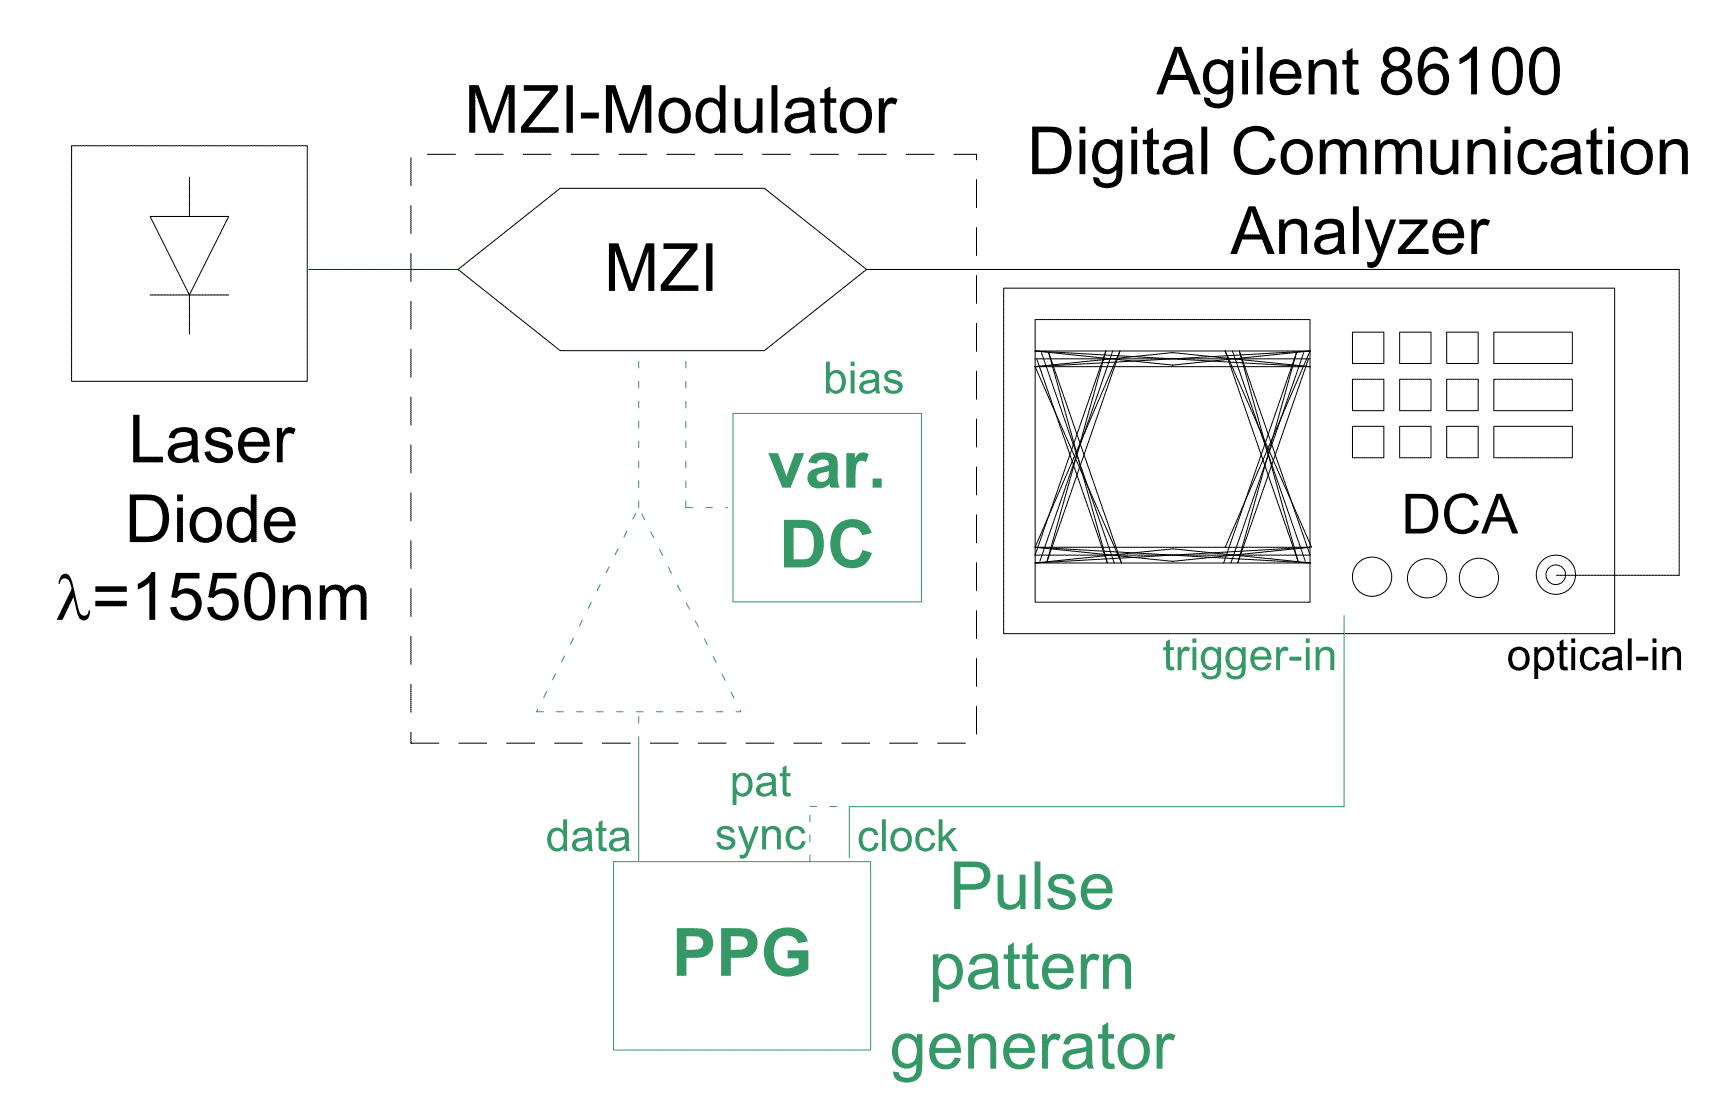
\includegraphics[width=.6\columnwidth]{Grafiken/B_setup.png}%
\caption{Setup B}%
\label{fig:B_setup}%
\end{figure} 

To determine the effect of the laser power on the extinction ratio (ratio of the optical power of the mark and the space) the laserpower was changed from one to 4~mW in steps of 1~mW. 

\begin{table}%
\centering
\caption{Extinction ratio for different laser powers}
 
\begin{tabular}{ccc}
\toprule
$P$~/~mW	& Extinction ratio~/dB\\
&min&max\\
\midrule
1 &9.16&9.2\\
2 &9.1&9.11\\
3 &9.19&9.22\\
4 &9.12&9.2\\
\bottomrule 
\end{tabular}
\label{tab:B_power}
\end{table}
Table \ref{tab:B_power} includes the measured maximum and minimum extinction ratios for the different laser powers. The change of the power shows no influence on the extinction ratio. Therefore an optical laserpower of 1.0~mW was used.

A change of amplitude of the clock between 1~V and 2~V showed that the highest extinction ration could be achieved at an voltage of 1.5~V. Changing the optical amplitude of the electrical data pulses showed that for an amplitude of 0.5~V the extinction ratio becomes small ($\sim 5.31$~dB). A higher amplitude of 1.5~V leads only to a small improvement. For that reason the amplitude of the data pulses was set to 1.0~V like in the task\footnote[3]{Luca Alloatti, Materials for the preparation of OKT lab 8} described.

Now at the pulse pattern generator (PPG) was set into the WORD mode to send a defined bit pattern. The generator was set to send the bit sequence ``00100100''. The PAT SYNC output of the PPG was connected to the front panel input of the oscilloscope.

Using the oscilloscope mode and the histogram option of the Agilent 86100 Digital Communication Analyzer the mean value and the standard deviation for both mark ($\mu_1,~\sigma_1$) and space ($\mu_0,~\sigma_0$) were estimated at the center of the pulse at a width of 10~\% of the pulse width. These values are shown in table \ref{tab:B_Q}.

\begin{table}%
\centering
\caption{Measured mean values and standard deviation and calculated Q-factors and bit error rate.}
 
\begin{tabular}{lcc}
\toprule
&mark&space\\
\midrule
mean value / $\upmu$W&105.5	&12.58	\\
standard deviation / $\upmu$W&11.4	&10.8	\\\midrule
Q-factor&	&	4.2\\
Q$^2$-factor / dB	&	&12.4\\
bit error rate	&	&$1.4\cdot 10^{-5}$\\
\bottomrule 
\end{tabular}
\label{tab:B_Q}
\end{table}

Using 
\begin{equation}
\begin{split}
\mathrm{Q} = \frac{\mu_1-\mu_0}{\sigma_1+\sigma_0}\\
\mathrm{Q}^2|\i{dB} = 10\cdot \mathrm{log}\left(\mathrm{Q}^2\right)
\label{eq:}
\end{split}
\end{equation} 
the linear Q-factor and the logarithmic Q$^2$ factor can be calculated. The \textit{BER} can be calculated with

\begin{equation}
BER = \frac{1}{2}\mathrm{erfc}\left(\frac{Q}{\sqrt{2}}\right)\qquad.
\label{eq:B_ber}
\end{equation}
Since the histograms of both mark and space were symmetric and looked Gaussian and therefore can be assumed to be Gaussian distributed and because the standard deviation of mark and space are nearly the same equation \eqref{eq:B_ber} can be used.

The calculated values can be found in table \ref{tab:B_Q}. The MZM seems not to be driven at its optimum. In the following task this becomes a problem and the operational settings are changed to achieve results using setup C.


\newpage
\section{Setup C: Reciever Sensitivity Measurement}


\begin{adjustwidth}{-2cm}{2cm}
\begin{figure}%
\centering
	\subfloat[]{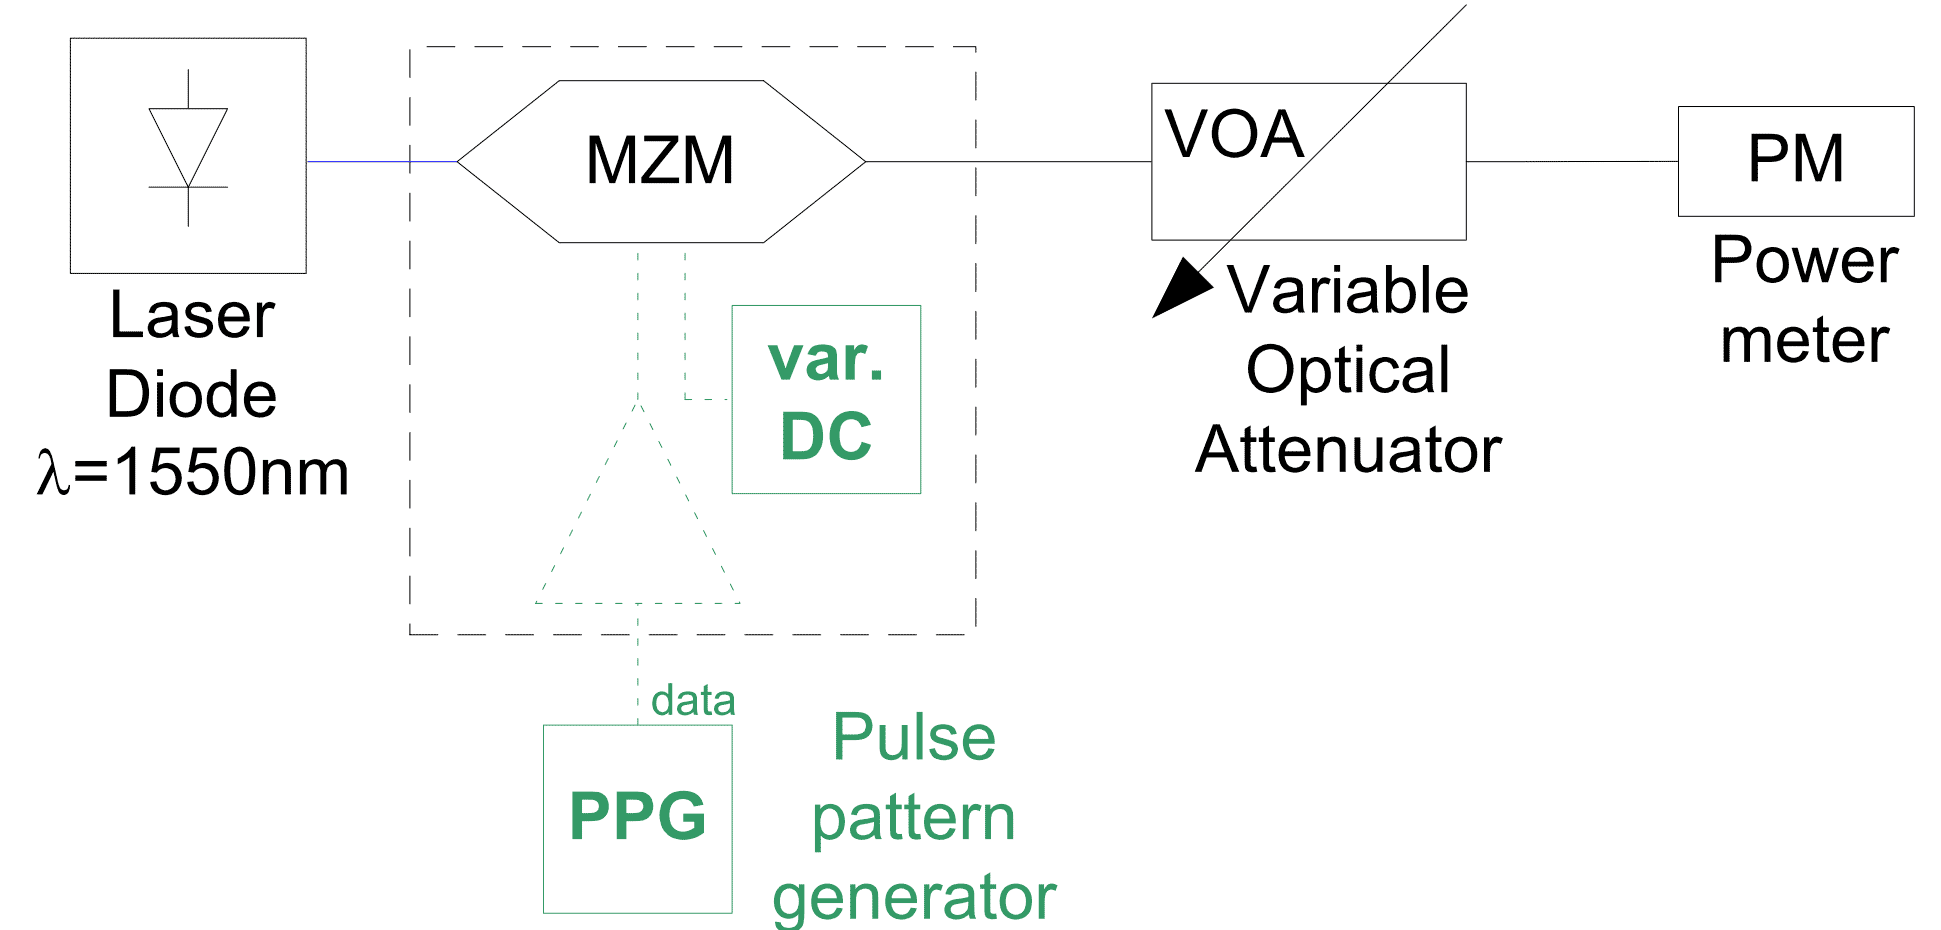
\includegraphics[width=.5\columnwidth]{Grafiken/C_setup1.png}\label{fig:C_setup1}}~~~~~~~~~
	\subfloat[]{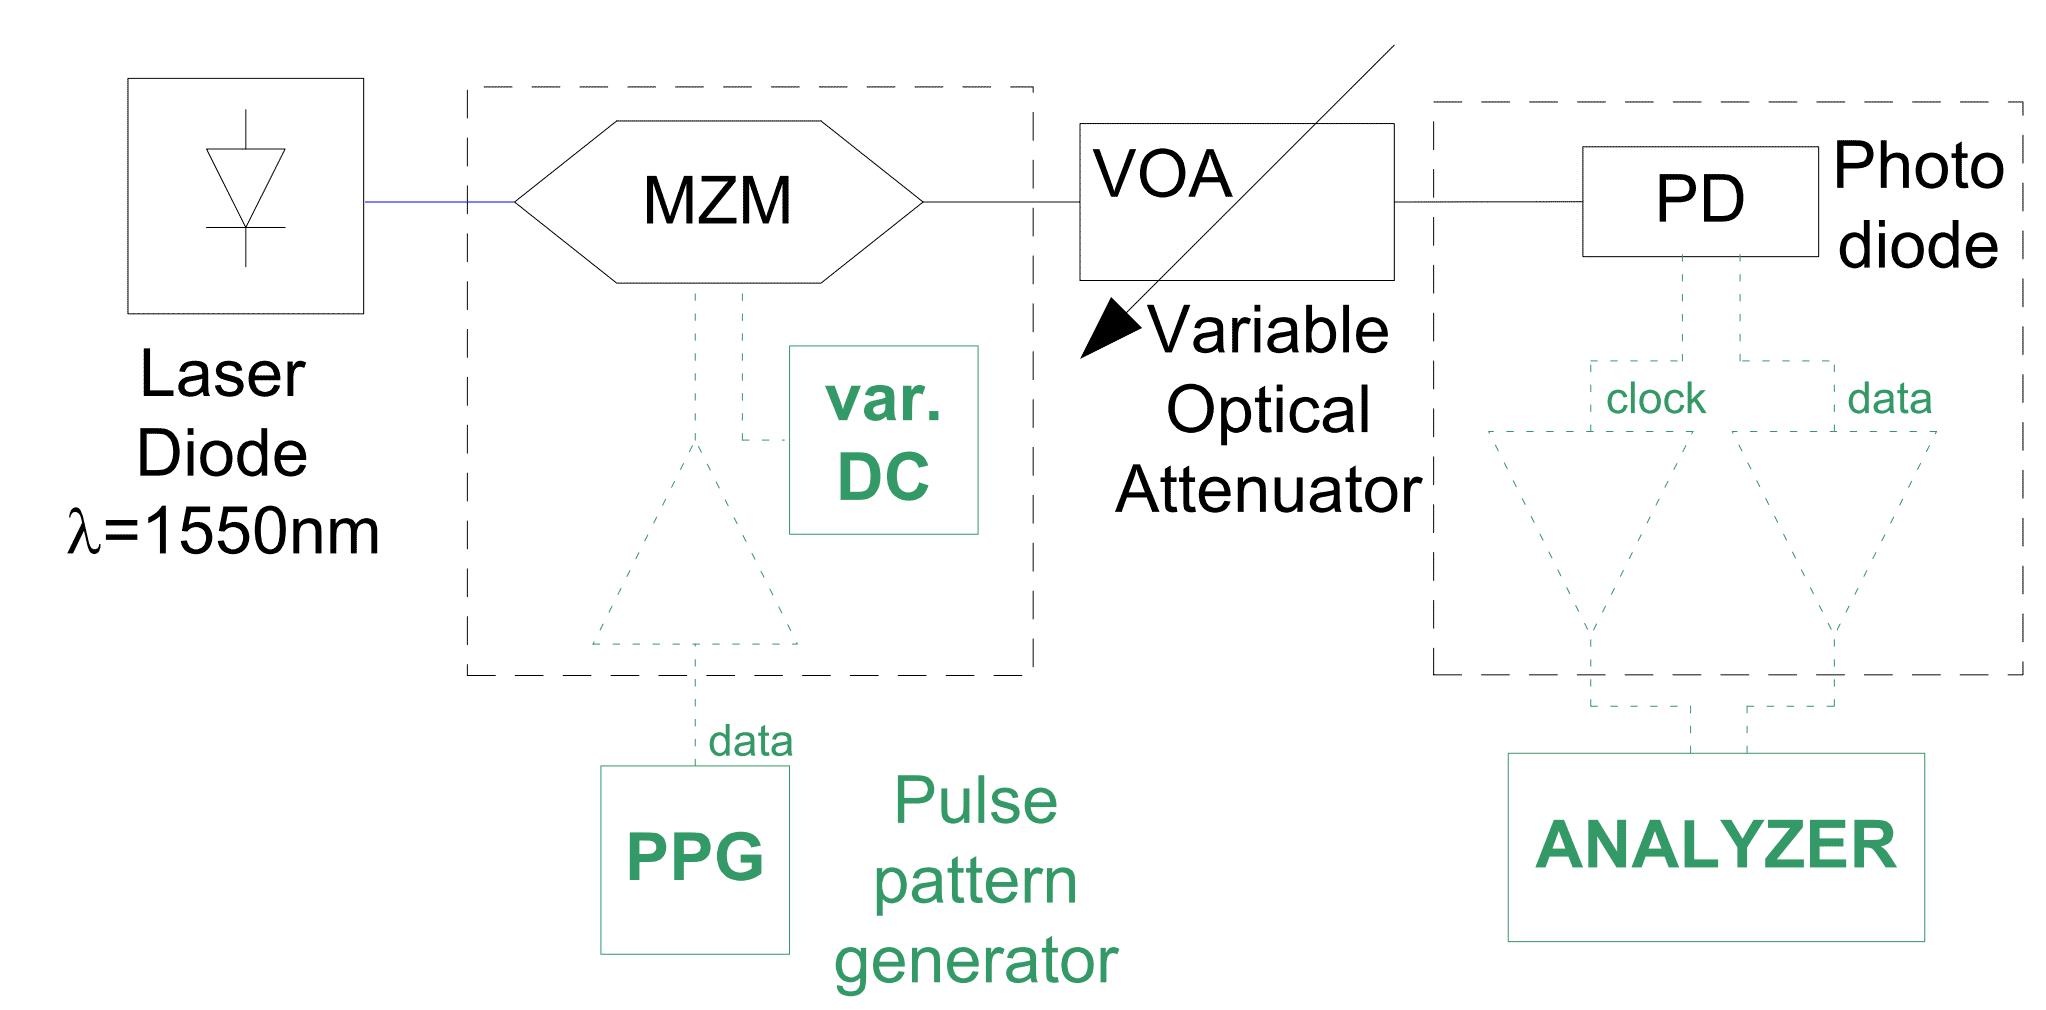
\includegraphics[width=.5\columnwidth]{Grafiken/C_setup2.png}\label{fig:C_setup2}}%
\caption{Setup C for the first part (a) and the second part (b)}%
\label{fig:13_42}%
\end{figure}
\end{adjustwidth}



The MZM was connected to a variable optical attenuator set to the lowest possible attenuation. Then the output power was measured using the connected power meter. Figure \ref{fig:C_setup1}\footnote[3]{Luca Alloatti, Materials for the preparation of OKT lab 8} shows the used setup. For a laser output power of 0~dBm the output power was measured to be 63.5~$\upmu$W.

In the next step the power meter was disconnected and the photo receiver connected like shown in figure \ref{fig:C_setup2}\footnotemark[3]. The $DATA$ and the $CLOCK$ electrical outputs of the photo reciever were connected to the corresponding inputs of the BER analyzer. At the pulse pattern generator PRBS was set as the data signal. The BER analyzer was set to $AUTOSEARCH$ in the $TIMED$ test mode. 






Using the settings used before (laserpower: 1~mW, electrical amplitude DATA: 1.0~V, electrical amplitude CLOCK: 1.5~V) lead to no measurable BERs. The BER analyzer showed ''NO DATA``. This could be caused by the fact, that the used settings were not in the optimal operation point of the MZM (cf. tab. \ref{tab:B_Q}). For that reason the operation point was re adjusted. The polarizers right after the laser were adjusted again and the output power of the laser was now set to 3~mW. This corresponds to a power of 0.382~mW at the output of the MZM. The DC bias voltage was set to -0.22~V and the DC amplitude to 1.15~V. At this operation point there was a big eye in the eye diagram.

With the variable optical attenuatior the power at the photo diode was varied and the BER was measured. Figure \ref{fig:BER} shows the dependence of the BER on the optical power for a bit squences of the length \textit{PN~17} and \textit{PN~20}, respectively.
 
In the \textit{PN~17} bit sequence one can see, that the BER decreases with increasing power. This can be explained by the fact that the signal in the optical transmission system is a poisson process. When the power is doubled the noise only increases by a factor of $\sqrt{2}$.

For the \textit{PN~20} bit sequence the bit error rate was in the magnitude of $10^{-5}$ indepenent from the input power. This behavior should not be caused by physical reasons. It is probably caused by faults of the BER analyzer system. It often didn't recognize the type of the bit sequence properly (``No Signal''), so that the measurement stoped and started again after a short period of time. Because of that, there were not always enough bit errors to determine the BER with a good accuracy.

The BER sensitivity of the photodetector is defined as the power level when a BER of $10^{-9}$ is reached at the reciver. Due to faults in the measurement system this value could not be reached. Thus the BER sensitivity could not be determined.


\begin{figure}%
\centering
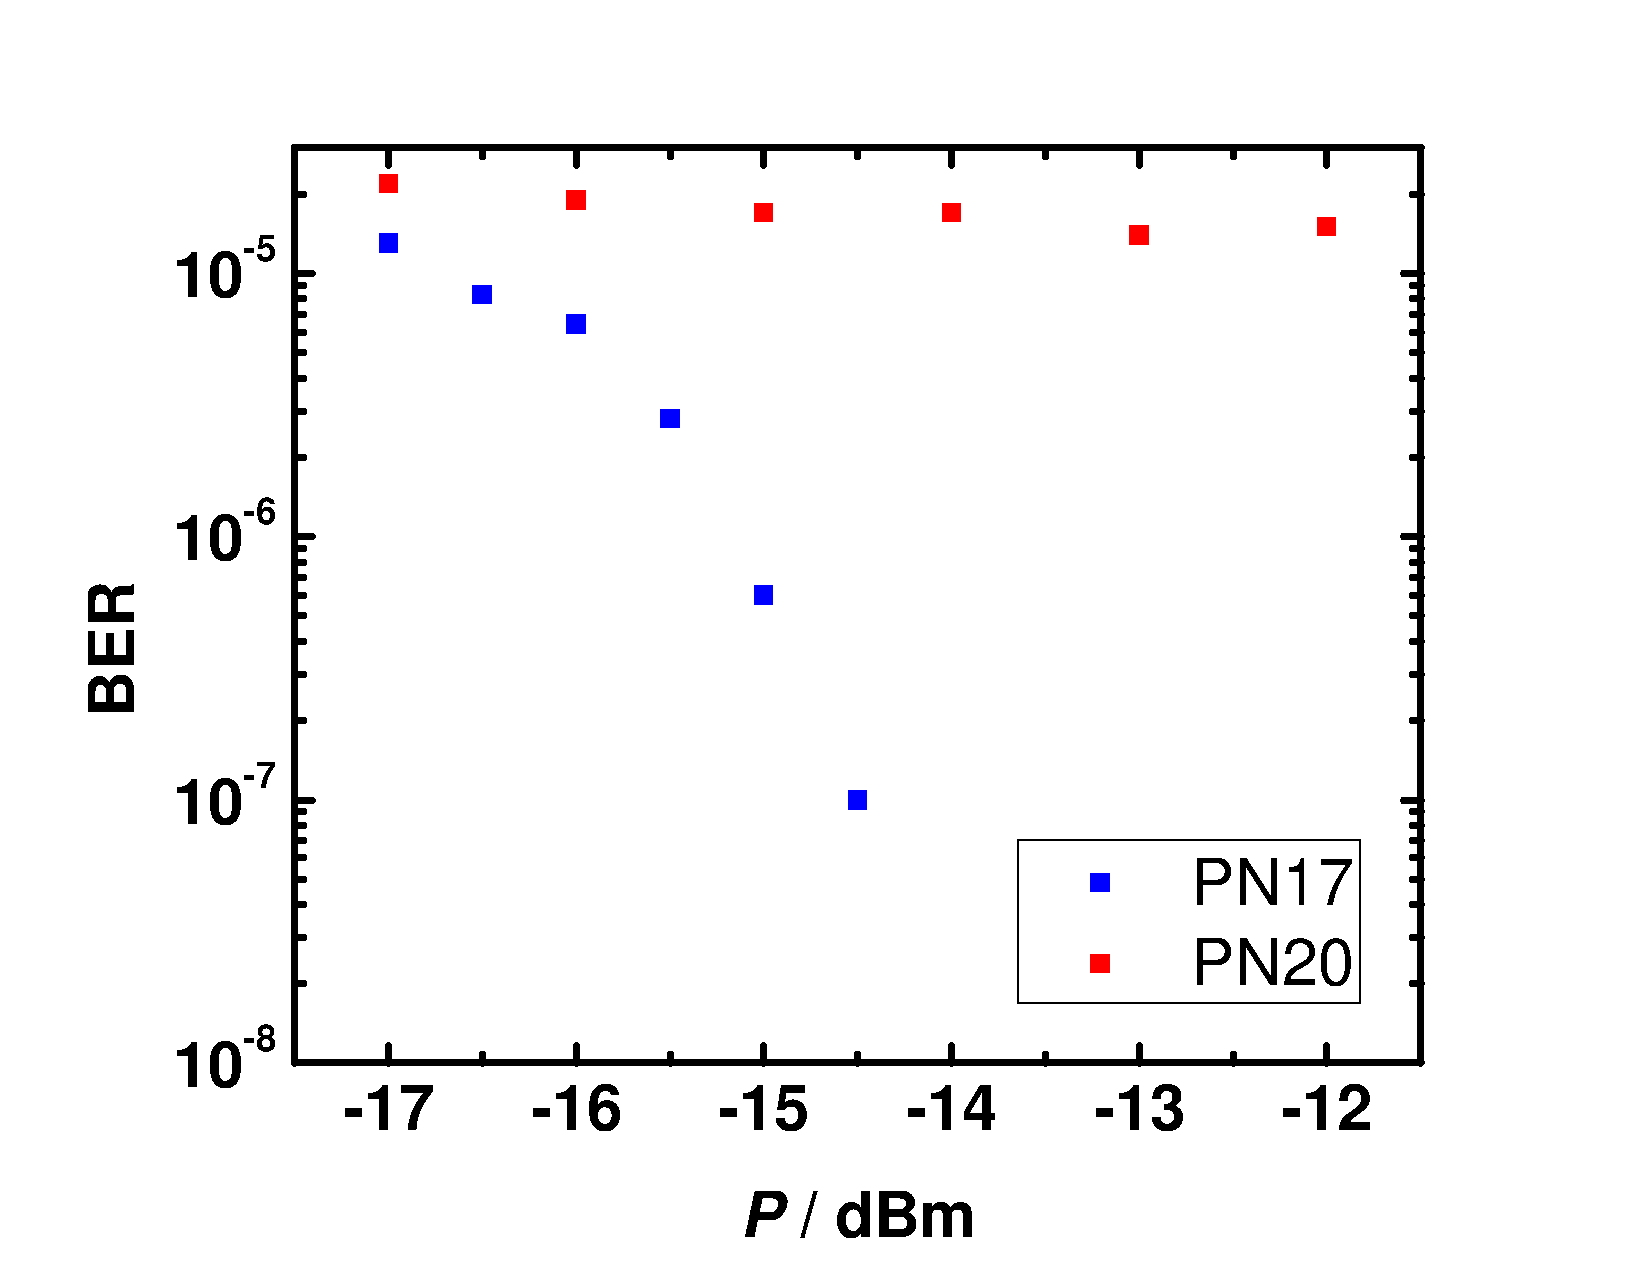
\includegraphics[width=.6\columnwidth]{Grafiken/BER.pdf}%
\caption{BER for different bit patterns.}%
\label{fig:BER}%
\end{figure}
